
\documentclass[11pt, a4paper]{article}
%\usepackage{proj1}
\usepackage{natbib}
\usepackage{fancyhdr}  
\usepackage{subcaption}
\usepackage{caption}
\usepackage{graphicx}
\usepackage{numprint}
\usepackage{multirow}
\linespread{1.25} 
\setlength{\parindent}{0cm}
\graphicspath{{Images/}}
\usepackage{hyperref}
\usepackage{amsmath}
\usepackage{amsfonts}
\usepackage{amssymb}
\usepackage{amsthm}
\usepackage{mathtools}
\usepackage{commath}
\usepackage{bbm}

%\usepackage[sc,osf]{mathpazo}
\usepackage{subcaption}
\usepackage[a4paper, top=1in, left=1.0in, right=1.0in, bottom=1in, includehead, includefoot]{geometry} %Usually have top as 1in

\usepackage{listings}
\usepackage{color} %red, green, blue, yellow, cyan, magenta, black, white
\definecolor{mygreen}{RGB}{28,172,0} % color values Red, Green, Blue
\definecolor{mylilas}{RGB}{170,55,241}


\hypersetup{colorlinks,linkcolor={black},citecolor={blue},urlcolor={black}}
\usepackage{color}
\urlstyle{same}


\theoremstyle{definition}
\newtheorem{definition}{Definition}[section]

\newcommand{\adja}{q_a}
\newcommand{\adjb}{q_b}
\newcommand{\adjaB}{q_{a,\partial \Omega}}
\newcommand{\adjbB}{q_{b,\partial \Omega}}
\newcommand{\adjB}{q_{\partial \Omega}}
\newcommand{\Adja}{\mathbf{p}}
\newcommand{\Adjb}{q}
\newcommand{\adj}{q}
\newcommand{\Adjc}{{q}_{\partial \Omega}}
\newcommand{\ra}{\rho_a}
\newcommand{\rb}{\rho_b}
\newcommand{\w}{\mathbf{w}}
\newcommand{\f}{\mathbf{f}}
\newcommand{\ve}{\mathbf{v}}
\newcommand{\n}{\mathbf{n}}
\newcommand{\h}{\mathbf{h}}
\newcommand{\K}{\mathbf{K}}
\newcommand{\hr}{\widehat \rho}
\newcommand{\jf}{\mathbf j}

\DeclareMathOperator{\sgn}{sgn}
\DeclareMathOperator{\Grad}{Grad}
\DeclareMathOperator{\Div}{Div}
\DeclareMathOperator{\Lap}{Lap}
%	\begin{figure}[h]
%		\centering
%		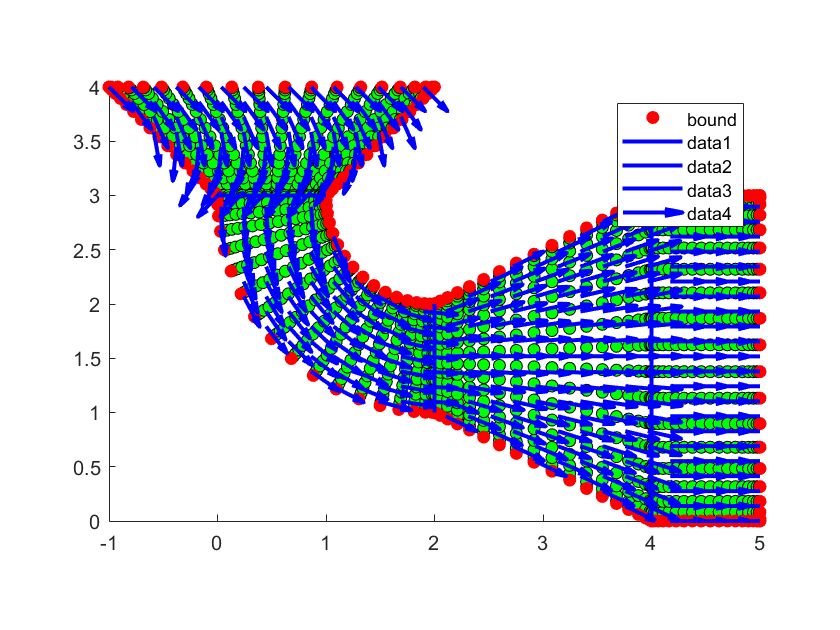
\includegraphics[scale=0.35]{F1.png}
%		\caption{Forward $\rho$ for $a = 0.01$} 
%		\label{F1}
%	\end{figure}

\begin{document}
	\section{Comparing to N-K}
Dirichlet interacting problem with $N = 20$, $\kappa = 1$, gives a difference of $1.5917 \times 10^{-11}$. The timings are $190$ s (NK) and $800$ s (FP).
Neumann interacting gives $4.1295 \times 10^{-12}$. Timings are $740$ s (NK), $490$ s (FP) Why is this timing so different?\\
Neumann and Dirichlet AD exact problems are the same to $10^{-15}/ 10^{-16}$ and so is the Dirichlet AD $+ V_{ext}$ problem.\\
For Paper Example 1 (2D) we get an error of $0.0014$ with $N = 30$ and $n = 20$. For $N = 20$, $n = 11$, the error is $0.0874$. Both errors increase when the relative instead of the absolute error is taken.\\
For Paper Example 1(1D) we get an error of $0.0037$, for $n = 30$ and $N = 50$ (and same for smaller $n$/$N$). The relative error is large. For $\kappa = 0$, the error is $10^{-13}$. 


\section{1D Problems}
The Dirichlet exact problem is solved with $N = 20$ and $n = 10$ in $3$ seconds. The error in $u$ and $v$ decreases down to the order of $10^{-15}$.
The Neumann exact problem is solved with $N = 30$ and $n = 19$ in $15$ seconds. The error in $u$ and $v$ decreases down to the order of $10^{-5}$, which is very different from the Dirichlet problem. The same happens in the 2D case. The inner number of iterations goes up to $100$ in the later outer iterations. However, this does not happen if I choose $N = 20$ and $n = 10$ and the error even decreases down to $10^{-12}$. In general, the more points I use, the worse the error gets. This is also the case for the Dirichlet problem, but it remains reasonably accurate despite this, while the Neumann problem is only accurate to $10^{-2}$ or similar for high numbers of points. In particular, this happens when we increase $n$, increasing $N$ does not seem to be the issue.
\\
\\
I then apply this observation to one of the paper examples (Example 2), with $\kappa = 1$. When I run the problem with $N = 50$ and $n = 10$, and then with the old code with $n = 30$ and interpolate to $n = 10$ in time, We get an error of $0.0362$. If I run both versions with $n = 30$ we get an error of $3.8640 \times 10^{-4}$, which seems to contradict the above observation. \\
For $n = 30$, we get for $\kappa =-1$ and error of $0.0013$ and for $\kappa = 0$ and error of $1.2519 \times 10^{-8}$. These problems take $56$ seconds to solve.
\\
\\
For the paper example 1, we again choose $N = 50$ and $n = 30$. We get for $\kappa = 0$ an error of $1.5563 \times 10^{-13}$, for $\kappa = -1$ we have the error $0.0174$ and for $\kappa = 1$, the error is $0.0037$.
\\
\\
For the third example, we have Dirichlet BCs and again choose $N = 50$ and $n = 30$. We get for $\kappa = 0$ the eroor is $1.8015 \times 10^{-7}$, for $\kappa = -1$ the error is $1.6645 \times 10^{-7}$ and for $\kappa  =1$ the error is $1.9485 \times 10^{-7}$.


\section{2D Problems}


\section{$H_1$ control and similar}
In the book Perspectives in flow control and optimization, Chapter 2, by Gunzburger the author poses a problem with a control including a gradient, see Figure \ref{F1}. The derivation shows the resulting no-flux boundary condition for the control.

	\begin{figure}[h]
		\centering
		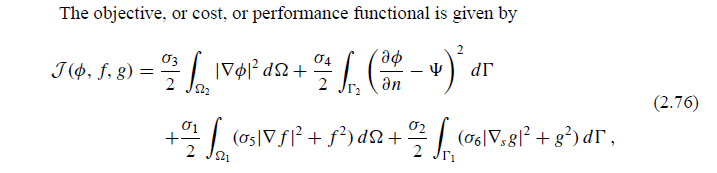
\includegraphics[scale=0.7]{Cost.png}
		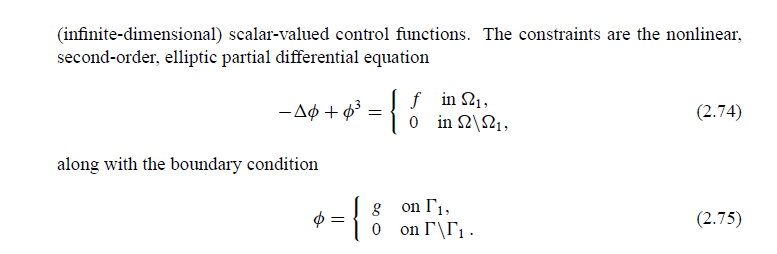
\includegraphics[scale=0.7]{Constraint.png}
		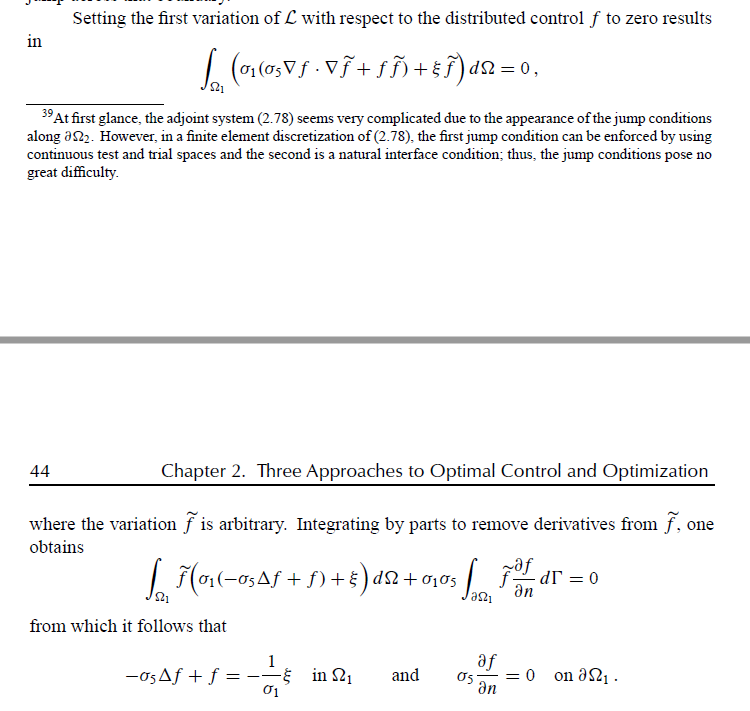
\includegraphics[scale=0.7]{GradientEqn.png}
		\caption{Gunzburger Book Result} 
		\label{F1}
	\end{figure}

The paper 'Optimal Control of Obstacle Problems by H1-Obstacles' by Ito is concerned with $H_1$ regularization, but as far as I can tell, neglects all boundary conditions.
In the paper 'Parallel Multiscale Gauss Newton Krylov Methods for Inverse Wave Propagation', the control is a gradient. They do apply no-flux boundary conditions, but state that they 'assume' them, rather than derive them.
The paper 'Image Sequence Interpolation Based on Optical Flow, Segmentation, and Optimal Control' has a gradient regularizer, for which Dirichlet boundary conditions are assumed in the optimality system.



The paper by Mang et al 'Constrained H1 Regularization Schemes for Diffeomorphic Image Registration' proposes a different way of enforcing a divergence free flow, see Figure \ref{F2}. They set periodic boundary conditions, which I cannot see to be derived in the process of getting the optimality system. They mention ill-posedness issues for $\nabla \cdot v = 0$, but I don't know what they would be/ if that applies to us.
	\begin{figure}[h]
	\centering
	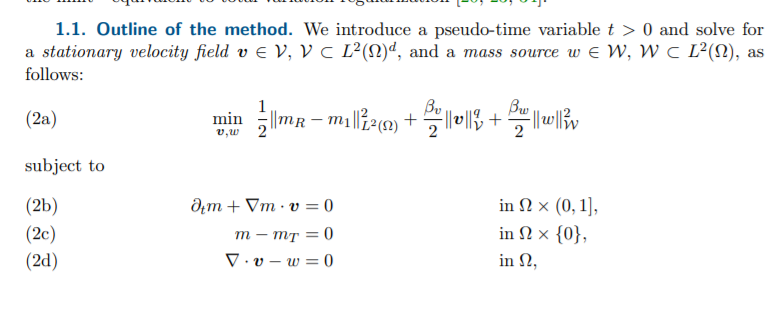
\includegraphics[scale=0.7]{Mang.png}
	\caption{Mang} 
	\label{F2}
\end{figure}
%@book{GunzburgerMaxD2003Pifc,
%	series = {Advances in design and control ; 5},
%	publisher = {Society for Industrial and Applied Mathematics (SIAM, 3600 Market Street, Floor 6, Philadelphia, PA 19104)},
%	isbn = {9780898718720},
%	year = {2003},
%	title = {Perspectives in flow control and optimization},
%	language = {eng},
%	address = {Philadelphia, Pa.},
%	author = {Gunzburger, Max D},
%	keywords = {Fluid dynamics -- Mathematics; Numerical analysis; Mathematical optimization},
%}

\end{document}